% This is a Basic Assignment Paper but with like Code and stuff allowed in it, there is also url, hyperlinks from contents included. 

\documentclass[11pt]{article}

% Preamble

\usepackage[margin=1in]{geometry}
\usepackage{amsfonts, amsmath, amssymb}
\usepackage{fancyhdr, float, graphicx}
\usepackage[utf8]{inputenc} % Required for inputting international characters
\usepackage[T1]{fontenc} % Output font encoding for international characters
\usepackage{fouriernc} % Use the New Century Schoolbook font
\usepackage[nottoc, notlot, notlof]{tocbibind}
\usepackage{listings}
\usepackage{xcolor}
\usepackage{blindtext}
\usepackage{hyperref}
\hypersetup{
    colorlinks=true,
    linkcolor=black,
    filecolor=magenta,      
    urlcolor=cyan,
    pdfpagemode=FullScreen,
    }

\definecolor{codegreen}{rgb}{0,0.6,0}
\definecolor{codegray}{rgb}{0.5,0.5,0.5}
\definecolor{codepurple}{rgb}{0.58,0,0.82}
\definecolor{backcolour}{rgb}{0.95,0.95,0.92}

\lstdefinestyle{mystyle}{
    backgroundcolor=\color{backcolour},   
    commentstyle=\color{codegreen},
    keywordstyle=\color{magenta},
    numberstyle=\tiny\color{codegray},
    stringstyle=\color{codepurple},
    basicstyle=\ttfamily\footnotesize,
    breakatwhitespace=false,         
    breaklines=true,                 
    captionpos=b,                    
    keepspaces=true,                 
    numbers=left,                    
    numbersep=5pt,                  
    showspaces=false,                
    showstringspaces=false,
    showtabs=false,                  
    tabsize=2
}

\lstset{style=mystyle}

% Header and Footer
\pagestyle{fancy}
\fancyhead{}
\fancyfoot{}
\fancyhead[L]{\textit{\Large{Advanced Data Structures - Assignment 4}}}
%\fancyhead[R]{\textit{something}}
\fancyfoot[C]{\thepage}
\renewcommand{\footrulewidth}{1pt}



% Other Doc Editing
% \parindent 0ex
%\renewcommand{\baselinestretch}{1.5}

\begin{document}

\begin{titlepage}
    \centering

    %---------------------------NAMES-------------------------------

    \huge\textsc{
        MIT World Peace University
    }\\

    \vspace{0.75\baselineskip} % space after Uni Name

    \LARGE{
        Advanced Data Structures\\
        Second Year B. Tech, Semester 4
    }

    \vfill % space after Sub Name

    %--------------------------TITLE-------------------------------

    \rule{\textwidth}{1.6pt}\vspace*{-\baselineskip}\vspace*{2pt}
    \rule{\textwidth}{0.6pt}
    \vspace{0.75\baselineskip} % Whitespace above the title



    \huge{\textsc{
            Implementation of Threaded Binary Tree and Its Traversals
        }} \\



    \vspace{0.5\baselineskip} % Whitespace below the title
    \rule{\textwidth}{0.6pt}\vspace*{-\baselineskip}\vspace*{2.8pt}
    \rule{\textwidth}{1.6pt}

    \vspace{1\baselineskip} % Whitespace after the title block

    %--------------------------SUBTITLE --------------------------	

    \LARGE\textsc{
        Assignment No. 4
    } % Subtitle or further description
    \vfill

    %--------------------------AUTHOR-------------------------------

    Prepared By
    \vspace{0.5\baselineskip} % Whitespace before the editors

    \Large{
        Krishnaraj Thadesar \\
        Cyber Security and Forensics\\
        Batch A1, PA 20
    }


    \vspace{0.5\baselineskip} % Whitespace below the editor list
    \today

\end{titlepage}

\tableofcontents
\thispagestyle{empty}
\clearpage

\setcounter{page}{1}

\section{Objectives}
\begin{enumerate}
    \item \textbf{To study the data Structure }: Threaded Binary Tree
    \item To study the advantages of Threaded Binary Tree over Binary Tree
\end{enumerate}

\section{Problem Statement}
Implement threaded binary tree and perform inorder traversal.

\section{Theory}
\subsection{Threaded Binary Tree}

\subsubsection{What is Threaded Binary Tree?}

\begin{figure}[H]
    \centering
    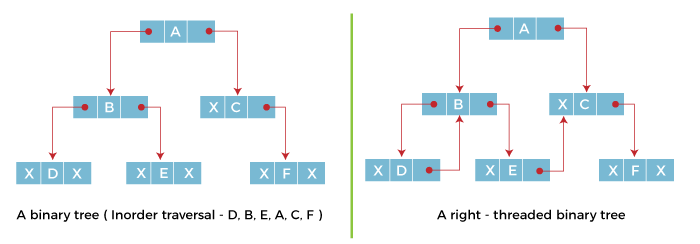
\includegraphics[width=1\textwidth]{figures/threaded-binary-tree3.png}
    \caption{Threaded and a Normal Binary Tree}
\end{figure}

\textit{A Threaded Binary Tree is a binary tree where every node has an extra bit, and this bit is used to indicate whether the right pointer points to the right child or to the inorder successor of the node. In this way, we can traverse the tree without using the stack and without recursion. A Threaded Binary Tree is a binary tree where every node has an extra bit, and this bit is used to indicate whether the right pointer points to the right child or to the inorder successor of the node. In this way, we can traverse the tree without using the stack and without recursion.}

\subsubsection{Advantages of Threaded Binary Tree}

\begin{enumerate}
    \item Threaded Binary Tree is used to traverse the tree without using the stack and without recursion.
    \item Inorder traversal of a binary tree is the most frequently used traversal. Inorder traversal of a threaded binary tree is done without using the stack and without recursion easier than the normal binary tree.
\end{enumerate}


\subsection{Space Utilization in Threaded Binary Tree}

\textbf{Space Utilized by a Normal Tree}
A Normal Binary Tree with N nodes each has data, left and right pointers. So, the space utilized by a normal binary tree is 3N.\

\textbf{Space Utilized by a Threaded Tree}

A Threaded Binary Tree with N nodes each has data, left and right pointers and 2 bits. So, the space utilized by a threaded binary tree is 3N+2N = 5N.\\

But they avoid the usege of a stack during traversal. So, the space utilized by a threaded binary tree is less than the space utilized by a normal binary tree.

\section{Platform}
\textbf{\textbf{Operating System}}: Arch Linux x86-64 \\
\textbf{\textbf{IDEs or Text Editors Used}}: Visual Studio Code\\
\textbf{\textbf{Compilers} }: g++ and gcc on linux for C++\\

\section{Input}
\begin{enumerate}
    \item Input at least 10 nodes.
    \item Display inorder traversal of binary tree with 10 nodes.
\end{enumerate}

\section{Output}
\begin{enumerate}
    \item The traversal of the Threaded binary tree in different ways.
\end{enumerate}

\section{Test Conditions}
\begin{enumerate}
    \item Input at least 10 nodes.
    \item Display all traversals of binary tree with 10 nodes.(recursive and nonrecursive)
\end{enumerate}

\section{Pseudo Code}
\subsection{Create}
\begin{lstlisting}[language=C++]
// Allocate memory for root
root = new ThreadedBinaryTreeNode()

// Assign root->leftc and rightc to head
root->left = head
root->right = head

// Accept root data
print "Enter the root data: "
cin >> root->data

// Assign head lbit to 0
head->left = root
// Assign head->leftc to root
head->isLeftNodeAThread = false

ThreadedBinaryTreeNode *temp, *curr
temp = root
bool flag = true
int again = 0
int choice = 0

print "Do you want to enter another node? (1 or 0)" << endl
cin >> again
while (again != 0)
    temp = root
    flag = true
    print "Enter 1 for Entering a new node to the Left, and 2 for Entering it to the right" << endl
    cin >> choice
    while (flag)
        if (choice == 1)
            if (temp->isLeftNodeAThread == true)
                curr = new ThreadedBinaryTreeNode()
                print "Enter the Data: "
                cin >> curr->data
                curr->right = temp
                temp->left = curr
                temp->isLeftNodeAThread = false
                flag = false
            else
                temp = temp->left
            
        else if (choice == 2)
            if (temp->isRightNodeAThread == true)
                curr = new ThreadedBinaryTreeNode()
                print "Enter the Data: "
                cin >> curr->data
                curr->left = temp
                curr->right = temp->right
                temp->right = curr
                temp->isRightNodeAThread = false
                flag = false
            else
                temp = temp->right
            
    print "Do you want to enter another node? (1 or 0)" << endl
    cin >> again

\end{lstlisting}
\subsection{Inorder Traversal}
\begin{lstlisting}[language=C++]
inorder_traversal()
    ThreadedBinaryTreeNode *temp
    temp = head
    while (true)
        temp = inorder_successor(temp)
        if (temp == head)
            break
        print temp->data << " "

ThreadedBinaryTreeNode *inorder_successor(ThreadedBinaryTreeNode *temp)
    ThreadedBinaryTreeNode *x = temp->right
    if (!temp->isRightNodeAThread)
        while (x->isLeftNodeAThread == false)
            x = x->left
    return x

\end{lstlisting}
\subsection{PreOrder Traversal}
\begin{lstlisting}[language=C++]
void preorder_traversal()
    ThreadedBinaryTreeNode *temp = head->left
    while (temp != head)
        print temp->data << " "
        while (temp->isLeftNodeAThread == false)
            temp = temp->left
            print temp->data << " "
        while (temp->isRightNodeAThread == true)
            temp = temp->right
        temp = temp->right

\end{lstlisting}

\section{Time Complexity}

\subsection{Creation of Threaded Binary Tree}
\begin{itemize}
    \item \textbf{Time Complexity:} O(n)
    \item \textbf{Space Complexity:} O(n)
\end{itemize}

\subsection{Inorder Traversal}

\begin{itemize}
    \item \textbf{Time Complexity:} O(n)
    \item \textbf{Space Complexity:} O(1)
\end{itemize}

\subsection{Preorder Traversal}

\begin{itemize}
    \item \textbf{Time Complexity:} O(n)
    \item \textbf{Space Complexity:} O(1)
\end{itemize}

\section{Code}

\subsection{Program}
\lstinputlisting[language=C++]{../Programs/Assignment_4.cpp}

\subsection{Input and Output}
\lstinputlisting[]{../Programs/Assignment_4_output.txt}

\section{Conclusion}
Thus, implemented threaded binary tree with inorder traversal.
\clearpage

\section{FAQ}
\begin{enumerate}
    \item \textbf{Why TBT can be traversed without stack?}\\

          A threaded binary tree is a binary tree that has additional links between nodes to allow for traversal without the use of a stack or recursion. These extra links, called threads, connect nodes that would otherwise be null pointers in a traditional binary tree.

          There \textbf{are two types of threaded binary trees}: inorder threaded binary trees and preorder threaded binary trees.

          \begin{enumerate}

              \item In an inorder threaded binary tree, the threads are used to connect nodes to their inorder predecessor and inorder successor. These threads allow for a traversal of the tree in inorder without using a stack or recursion. To traverse the tree in inorder without a stack, you start at the root node and follow the leftmost thread until you reach a node without a left child. Then, you visit that node and follow the thread to its inorder successor. You repeat this process until you have visited all nodes in the tree.

              \item In a preorder threaded binary tree, the threads are used to connect nodes to their preorder successor. These threads allow for a traversal of the tree in preorder without using a stack or recursion. To traverse the tree in preorder without a stack, you start at the root node and visit each node in the tree in preorder. When you visit a node, you follow the thread to its preorder successor and visit that node next.

              \item In both cases, the threads provide a way to traverse the tree without using a stack or recursion, which can be useful in situations where memory usage is a concern or where recursion or stack-based algorithms are not allowed. However, constructing the threads requires additional memory and processing time, so the benefits of threaded binary trees depend on the specific use case.
          \end{enumerate}

    \item \textbf{What are the advantages and disadvantages of TBT?}\\

          Threaded binary trees have several advantages and disadvantages that should be considered when deciding whether to use them in a specific scenario. Here are some of the main advantages and disadvantages:

          \textbf{Advantages}:

          \begin{enumerate}
              \item \textbf{Traversal without stack or recursion}: As mentioned before, threaded binary trees allow for traversal without using a stack or recursion. This can be useful in situations where memory usage is a concern or where recursion or stack-based algorithms are not allowed.

              \item \textbf{Efficient Inorder and Preorder Traversal}: The use of threads can significantly improve the performance of inorder and preorder traversal. In fact, threaded binary trees can perform these traversals in O(n) time complexity, which is faster than the O(nlogn) complexity of the recursive approach.

              \item \textbf{Space Efficiency}: Compared to traditional binary trees, threaded binary trees require less space to store the threads. This can be useful in situations where memory usage is a concern.

          \end{enumerate}
          \textbf{Disadvantages}:
          \begin{enumerate}


              \item \textbf{Construction Overhead}: The process of constructing threads can be time-consuming and requires additional memory. In some cases, the overhead of constructing the threads can negate any performance benefits.

              \item \textbf{Complexity}: Threaded binary trees can be more complex than traditional binary trees due to the additional links. This can make them harder to understand and maintain.

              \item \textbf{Limited Applications}: Threaded binary trees are not suitable for all types of problems. They are typically used in scenarios where traversal performance is critical, but in other cases, traditional binary trees or other data structures may be more appropriate.
          \end{enumerate}

    \item \textbf{Write application of TBT}\\

          \begin{enumerate}
              \item \textbf{Expression Trees}: Threaded binary trees can be used to represent arithmetic expressions in a compact form. By using threads, the expression tree can be traversed efficiently without using a stack or recursion. This can be useful in compilers and other applications that deal with arithmetic expressions.

              \item \textbf{Database Indexing}: Threaded binary trees can be used to implement indexing in databases. By using threads, the binary tree can be traversed efficiently, which can improve the performance of database queries.

              \item \textbf{Text Editors}: Threaded binary trees can be used in text editors to efficiently search for words in a document. By using threads, the binary tree can be traversed efficiently, which can improve the speed of searches.

              \item \textbf{Spell Checking}: Threaded binary trees can be used in spell checking applications to efficiently search for misspelled words. By using threads, the binary tree can be traversed efficiently, which can improve the speed of spell checking.

              \item \textbf{Image Processing}: Threaded binary trees can be used in image processing applications to efficiently process pixels in an image. By using threads, the binary tree can be traversed efficiently, which can improve the speed of image processing algorithms.

          \end{enumerate}

\end{enumerate}

\end{document}